\documentclass[a4paper,12pt, oneside]{book}

%\usepackage{fullpage}
\usepackage[T1]{fontenc}
\usepackage[italian]{babel}
\usepackage[utf8]{inputenc}
\usepackage{amssymb}
\usepackage{amsthm}
\usepackage{graphics}
\usepackage{amsfonts}
\usepackage{listings}
\usepackage{amsmath}
\usepackage{amstext}
\usepackage{engrec}
\usepackage{rotating}
\usepackage[safe,extra]{tipa}
\usepackage{showkeys}
\usepackage{multirow}
\usepackage{hyperref}
\usepackage{microtype}
\usepackage{enumerate}
\usepackage{braket}
\usepackage{marginnote}
\usepackage{pgfplots}
\usepackage{cancel}
\usepackage{polynom}
\usepackage{booktabs}
\usepackage{enumitem}
\usepackage{framed}
\usepackage{pdfpages}
\usepackage{pgfplots}
\usepackage[cache=false]{minted}
 \usepackage[usenames,dvipsnames, pdf]{pstricks}
 \usepackage{epsfig}
 \usepackage{pst-grad} % For gradients
 \usepackage{pst-plot} % For axes
 \usepackage[space]{grffile} % For spaces in paths
 \usepackage{etoolbox} % For spaces in paths
 \makeatletter % For spaces in paths
 \patchcmd\Gread@eps{\@inputcheck#1 }{\@inputcheck"#1"\relax}{}{}
 \makeatother
\usepackage{fancyhdr}
\pagestyle{fancy}
\fancyhead[LE,RO]{\slshape \rightmark}
\fancyhead[LO,RE]{\slshape \leftmark}
\fancyfoot[C]{\thepage}



\title{Analisi e Progettazione del Software}
\author{UniShare\\\\Davide Cozzi\\\href{https://t.me/dlcgold}{@dlcgold}\\\\Gabriele De Rosa\\\href{https://t.me/derogab}{@derogab} \\\\Federica Di Lauro\\\href{https://t.me/f_dila}{@f\textunderscore dila}}
\date{}

\pgfplotsset{compat=1.13}
\begin{document}
\maketitle

\definecolor{shadecolor}{gray}{0.80}

\newtheorem{teorema}{Teorema}
\newtheorem{definizione}{Definizione}
\newtheorem{esempio}{Esempio}
\newtheorem{corollario}{Corollario}
\newtheorem{lemma}{Lemma}
\newtheorem{osservazione}{Osservazione}
\newtheorem{nota}{Nota}
\newtheorem{esercizio}{Esercizio}
\tableofcontents
\renewcommand{\chaptermark}[1]{%
	\markboth{\chaptername
		\ \thechapter.\ #1}{}}
\renewcommand{\sectionmark}[1]{\markright{\thesection.\ #1}}
\chapter{Introduzione}
\textbf{Questi appunti sono presi durante le lezioni in aula. Per quanto sia stata fatta una revisione è altamente probabile (praticamente certo) che possano contenere errori, sia di stampa che di vero e proprio contenuto. Per eventuali proposte di correzione effettuare una pull request. Link: } \url{https://github.com/dlcgold/Appunti}.\\
\textbf{Grazie mille e buono studio!}
\chapter{Introduzione all'Ingegneria del software}
Durante il corso di Analisi e Progettazione del software si analizzano i modelli e i principi per lo sviluppo di un
software mantenibile, andando anche ad analizzare, in maniera sommaria, anche tutti gli strumenti di
ingegneria del software, necessari per lo sviluppo ottimale di un software.

In questo corso studieremo in dettaglio i seguenti argomenti:
\begin{itemize}
	\item introduzione all'ingegneria del software
	\item progettazione sistemi orientati ad oggetti
	\item modellazione a dominio
	\item UML e analisi dei casi d'uso
	\item design pattern
	\item sviluppo test-driven(cenni)
	\item code smell e refactoring(cenni)
\end{itemize}
Il software, è l'insieme delle componenti modificabili e non fisiche di un calcolatore, viene diviso in due categorie:
\begin{description}
	\item [generici], per un ampio range di clienti, come ad esempio gli elaboratori di testi
	\item [custom], per un singolo cliente, come ad esempio i gestionali specifici di un impresa
\end{description}
Questa differenza si sta sempre più assottiliando in quanto recentemente varie aziende stanno sviluppando un
software generico, che viene poi adattato in base alle esigenze del singolo cliente,
come ad esempio i software Oracle e Sas.

Nello sviluppo di software si utlizza spesso una base pre-esistente, infatti l'ingegneria del software si occupa
di tutti gli aspetti per lo sviluppo del software, sfruttando di solito una base preesistente. \newline
Di solito quando si sviluppa un software si presuppone che abbia una durata di alcuni anni, con la predispozione
al cambiamento e all'introduzione di nuove features infatti un software per essere utile deve essere continuamente cambiato.

Si hanno due tipologie di progetti:
\begin{enumerate}
	\item \textbf{progetti di routine}, con soluzione di problemi e riuso di vecchio codice
	\item \textbf{progetti innovativi}, con soluzioni nuovi
\end{enumerate}
e solitamente l'ingegneria del software si occupa principalmente di progetti innovativi
con specifiche del progetto variabili, con la presenza di cambiamenti continui e ovviamente
non è uguale nè similare con l'ingegneria tradizionale.

Un programmatore normalmente lavora da solo, su un programma completo con specifiche note mentre un ingegnere del software
lavora in gruppo, progetta componenti e l'architettura e identifica requisiti e specifiche.
Il costo del software spesso supera quello hardware %aggiungere grafico

Nello sviluppo di un software si hanno le seguenti fasi di sviluppo:
\begin{itemize}
	\item \textbf{analisi dei requisiti}, che indica cosa deve fare il sistema
	\item \textbf{progettazione}, progetto del sistema d implementare
	\item \textbf{sviluppo}, produzione del sistema software
	\item \textbf{convalida}, verifica dei requisiti del cliente
	\item \textbf{evoluzione}, evoluzione al cambiare di requisiti del cliente
\end{itemize}
Esistono dei sistemi software per l'automazione delle attività svolte nel progetto software,
i cosiddetti \textbf{CASE} (Computer-Aided Software Engineering) che si dividono in:
\begin{description}
	\item [CASE di alto livello] per il supporto alle prime attività di processo come la raccolta requisiti e la progettazione
	\item [CASE di basso livello] per il supporto alle ultime attività di processo come la programmazione,
	      il debugging, testing e reverse engineering
\end{description}
Nella figure X1 e X2  si hanno delle risposte alle comuni domande sull'ingegneria del software e le caratteristiche
di un ottimo software, necessario per mantenerlo facilmente modificabile nel tempo.

Nello sviluppo di un software, qualsiasi tipologia esso sia, prevede i seguenti aspetti in comune:
\begin{description}
	\item [specifiche del software] vengono definite le specifiche e analizzato in dettaglio il comportamento
	      e le funzionalità richieste da sviluppare
	\item [sviluppo del software] viene effettivamente implementato e progettato il codice, attraverso i tools di sviluppo,
	      rispettando le specifiche previste nella fase precedente.
	\item [convalida del software] viene testato il software sviluppato nella fase precedente, al f
	\item [evoluzione del software] viene mantenuto ed evoluto il software, al fine di riflettere i cambiamenti e delle
	      funzionalità richieste dal cliente;è la fase più critica e costosa, dato che a volte la manutenzione richiede
	      di sistemare e correggere gli errori e/o il cattivo design del progetto.
\end{description}
Il software deve essere accettato dagli utenti per i quali è stato sviluppato per cui deve essere comprensibile,
usabile e compatibile con altri sistemi, oltre a dover essere mantenibile, affidabile ma soprattutto efficente.

Esiste un codice etico, \textbf{ACM/IEEE}, con otto principi legati al comportamento degli ingegneri del software
ed è fondamentale seguirlo dato che fornisce informazioni su come risolvere i problemi etici collegati
a tutti i progetti software, come le informazioni da fornire all'esterno ed altri aspetti.

Un \textbf{sistema} è una collezione significativa di componenti interrelati che lavorano assieme per realizzare
un obiettivo comune, quindi include software e parti meccaniche o elettriche;inoltre si ha che i vari
componenti possono dipendere da altri componenti e che le proprietà e il comportamento dei vari componenti
sono intrinsecamente correlati, quindi si hanno due macro categorie:
\begin{enumerate}
	\item \textbf{sistemi tecnico-informatici}, in cui sono inclusi hardware e software ma non gli operatori e i
	      processi operazionali, dove sono presenti le \textbf{proprietà emergenti}, dipendenti dalle sue componenti
	      e le relazioni tra esse, misurabili soltanto sul sistema finale.\newline
	      Inoltre i sistemi tecnici sono non-deterministici, in quanto dato lo stesso input non è detto che restituisca
	      lo stesso output, in quanto il risultato è spesso dipendente dal comportamento degli operatori umani.
	\item \textbf{sistemi socio-tecnici}, comprendente uno o più sistemi tecnici, assieme ai processi operazionali
	      e agli operatori, sono fortemente condizionati da politiche aziendali e regole.\newline
	      I sistemi Socio-tecnici sono sistemi pensati per raggiungere obiettivi aziendali o organizzativi
	      e bisogna comprendere a fondo l'ambiente organizzatico nel quale un certo sistema è usato.
\end{enumerate}
Vediamo qualche proprietà emergente:
\begin{itemize}
    \item \textbf{volume:} il volume di un sistema varia a seconda di come sono disposti
        e collegati i componenti che lo formano.
    \item \textbf{affidabilità:} l'affidabilità del sistema dipende dall'affidabilità dei suoi componenti,
        ma interazioni impreviste possono produrre nuovi fallimenti 
        e quindi influenzare l'affidabilità dell'intero sistema
    \item \textbf{protezione:} la protezione del sistema è una proprietà complessa 
        che non può essere facilmente misurata, in quanto in futuro potrebbero essere inventati
        nuove modalità di accesso e/o attacco che rendeno meno protetto il software.
    \item \textbf{riparabilità:} questa proprietà riflette la facilità con cui è possibile
        correggere un problema e ciò dipende dalla possibilità di diagnosticare il problema
        e soprattutto di accedere, modificare o sostituire i componenti difettosi.
    \item \textbf{usabilità:} questa proprietà mostra la facilità d‘uso del sistema e dipende dai componenti del
            sistema tecnico, dai suoi operatori e dal suo ambiente operativo.
\end{itemize}
Oltre a questi sistemi software standard, sono presenti i \textbf{sistemi critici}, 
in cui fondamentalmente non sono ammessi errori e malfunzionamenti altrimenti causano dei gravi problemi
se non morti, per questo le specifiche avvengono in linguaggio il più possibile formale possibile
e usano un modello di sviluppo a cascata, inefficente per gli altri sistemi software.

Abbiamo tre esempi di sistemi critici:
\begin{enumerate}
    \item \textbf{sistemi safety-critical} dove i fallimenti comportano rischi ambientali
        o perdite di vite umane, come ad esempio un sistema di controllo per un impianto chimico.
    \item \textbf{sistemi mission-critical} dove i fallimenti possono causare il fallimento 
        di attività a obiettivi diretti, come un sistema di navigazione di un veicolo spaziale.
    \item \textbf{sistemi business-critical} dove i fallimenti possono risultare 
        in perdite di denaro sostenute, come ad esempio un sistema bancario.
\end{enumerate}
I fallimenti di un software, sia che fossero piccoli che grandi, possono essere di diversi tipi:
\begin{itemize}
	\item \textbf{fallimenti hardware}, errori di progetto, produzione o "consumo"
	\item \textbf{fallimenti software}, errori di specifica, progetto, implementazione
	\item \textbf{errori operativi}, errori commessi da operatori umani (forse una delle maggiori cause di fallimenti)
\end{itemize}
Nei sistemi critici, generalmente la fidatezza è la più importante proprietà del sistema 
in quanto si ha un alto costo dei fallimenti ed esso riflette il livello di confidenza
che l'utente ha verso il sistema, cosa leggermente diversa dall'utilità,
ossia la sicurezza di non avere problemi e/o intrusioni da parte di persone esterne.

Il costo dei fallimenti nei sistemi critici è così alto che i metodi di ingegneria del software
non sono cost-effective per cui si utilizza un modello a cascata, in quanto si devono fare prima 
tutte le analisi, prima di poter implementare e testare il sistema e soprattutto si spende un
sacco di soldi per il testing e le analisi per convalidare la fidatezza necessaria da raggiungere.

\section{Modelli di Processo}
Il modello di un processo software è una rappresentazione semplificata del processo, basata su un aspetto specifico:
\begin{itemize}
	\item \textbf{modello a flusso di lavoro (Workflow)} per una sequenza di attività
	\item \textbf{modello a flusso di dati (Data-flow)} per il flusso delle informazioni
	\item \textbf{modello ruolo/azione (role/action)} per decidere i vari ruoli
\end{itemize}
si hanno poi tre modelli generici:
\begin{enumerate}
    \item \textbf{modello a cascata (waterfall)}: modello in cui le diverse fasi, come si nota nella figura \figurename~\ref{fig:wf},
        avvengono  in sequenza, dove i problemi e/o mancanze di interpretazioni si notano verso 
        la fine dello sviluppo, nella fase di test e/o consegna, e ciò comporta una modifica di una 
        o più fasi precedenti dello sviluppo, con notevoli aggravi di costi e tempestiche.\newline
        È stato il primo modello di sviluppo, ma a partire dagli anni 90 si comprese che la 
        maggioranza dei fallimenti dei software era da imputare al fatto di cercare di definire tutti
        i requisiti prima di sviluppare, cosa che è difficile da fare in maniera efficace in sistemi 
        variabili nel tempo, come quasi tutti i sistemi software da sviluppare e/o già sviluppati.
        \begin{figure}
        	\centering
        	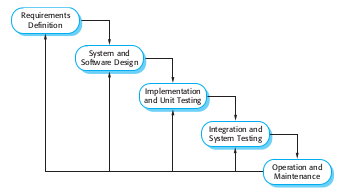
\includegraphics[scale=0.7]{img/wf.png}
        	\caption{Modello a cascata \label{fig:wf} }
        \end{figure}
        Vediamo una spiegazione più dettagliata:
        \begin{itemize}
        	\item \textbf{Requirements analysis and definition}: si stabiliscono servizi, limiti e fini del software consultandosi col cliente
        	\item \textbf{System and software design}: si stabilisce un'architettura di sistema complessiva stabilendo l'hardware e il software necessario
        	\item \textbf{Implementation and unit testing}: si sviluppano le unità di test e si verifica che ogni parte del software risponda alle specifiche richieste presa singolarmente
        	\item \textbf{Integration and system testing}: si testa il software nella sua interezza, si verifica che il software rispetti ogni requisito e infine si consegna il prodotto al cliente
        	\item \textbf{Operation and maintenance}: una volta che il prodotto è stato consegnato si provvede a mantenerlo, risolvendo eventuali errori e aggiungendo eventuali funzionalità, soddisfacendo eventuali nuovi requisiti. Potrebbe non essere uno step presente ogni volta
        \end{itemize}
    \item \textbf{modello iterativo (Iterative development)}: modello in cui le fasi di sviluppo avvengono
        nel corso del tempo, senza effettuare prima tutta la progettazione e poi l'implementazione, 
        sviluppando versioni sempre più definite del software, portando subito in risalta i problemi 
        e/o le mancate interpretazioni del sistema da sviluppare.\newline
        Prevede diverse implementazioni di questo modello, come ad esempio l'UP, lo Scrum e la modellazione
        agile, in cui il concetto di fondo è quello di conoscere, sviluppare e progettare il sistema a passi
        successivi, al fine di avere ad ogni passo un sottoinsieme del sistema già funzionante e questo
        permette di poter reagire ai cambiamenti dei requisiti e permettere una manutenzione
        mantenibile nel tempo.
    \item \textbf{ingegneria del Software basata sui componenti (CBSE)}
\end{enumerate}
\newpage
\subsubsection{Sviluppo incrementale}
Lo sviluppo incrementale si basa sull'idea di sviluppare un'implementazione iniziale del software che viene revisionata dai futuri utenti dello stesso. Si procede nella stessa maniera con ulteriori versioni fino a giungere ad un'implementazione finale. Quindi sviluppo, indicato in figura \figurename~\ref{fig:inc} e consegna sono strutturati in una sequenza di incrementi, ognuno delle quali corrisponde a parte delle funzionalità richieste, con ovviamente un ordine di priorità dato dal cliente (le prime parti conterranno le funzionalità principali del software).
\begin{figure}
	\centering
	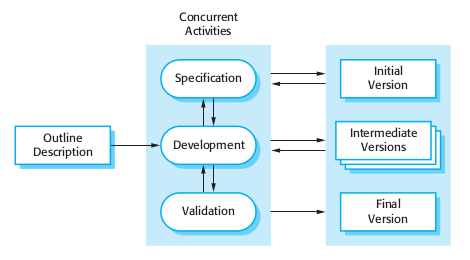
\includegraphics[scale=0.7]{img/inc.png}
	\caption{sviluppo incrementale \label{fig:inc} }
\end{figure}
Lo sviluppo incrementale ha 3 vantaggi principali rispetto 
al modello a cascata:
\begin{enumerate}
	\item si riduce il costo relativo al cambio di specifiche del cliente, riducendo anche la quantità di analisi e documentazione che andrebbe rielaborata
	\item si hanno feedback costanti sullo sviluppo grazie alla continua prova diretta delle varie implementazioni
	\item si può fornire gradualmente al cliente un software funzionante anche se privo di alcune features, di modo che possa usare parte del software ben prima del suo completo sviluppo
\end{enumerate}
Inoltre i rischi di fallimento si abbassano e i servizi a priorità più alta sono testati più a fondo. Del resto questo modello può essere rallentato facilmente da problemi burocratici. Inoltre il processo di sviluppo è più difficile da controllare da parte di un manager e il continuo aggiungere features può danneggiare l'architettura generale del software 
\textbf{pagina 34}










I metodi di ingegneria del software sono l'implementazione dei seguenti modelli generici, e nella
maggioranza si utilizza un modello iterativo, al fine di rendere incrementale lo sviluppo e ridurre
il rischio di fallimento del progetto.
\begin{center}
	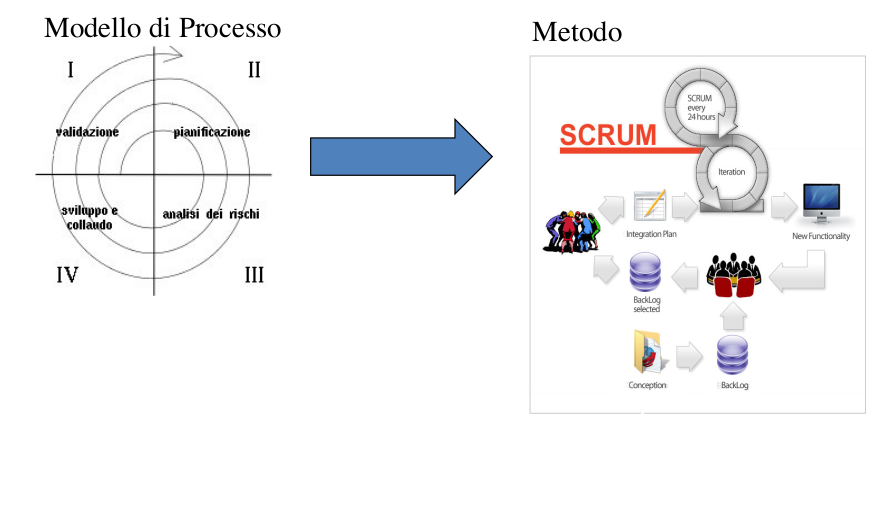
\includegraphics[scale=2.0]{img/ing.png}
\end{center}
% inizio sistemazione

si ha il seguente feedback del modello a cascata:
\begin{center}
\psscalebox{1.0 1.0} % Change this value to rescale the drawing.
{
\begin{pspicture}(0,-3.8)(15.6,3.8)
\psframe[linecolor=black, linewidth=0.04, dimen=outer](2.8,3.8)(0.0,2.6)
\psframe[linecolor=black, linewidth=0.04, dimen=outer](6.0,2.2)(2.8,1.0)
\psframe[linecolor=black, linewidth=0.04, dimen=outer](9.2,0.6)(6.0,-0.6)
\psframe[linecolor=black, linewidth=0.04, dimen=outer](12.4,-1.0)(9.2,-2.2)
\psframe[linecolor=black, linewidth=0.04, dimen=outer](15.6,-2.6)(12.4,-3.8)
\rput[bl](0.53333336,3.3){definizione}
\rput[bl](0.43333334,2.82){dei requisiti}
\rput[bl](2.8990476,1.76){progettazione}
\rput[bl](3.1866667,1.46){del sistema e}
\rput[bl](6.087619,0.0){implementazione}
\rput[bl](6.0804764,-0.44){e test delle unità}
\rput[bl](9.546667,-1.52){integrazione e }
\rput[bl](9.486667,-2.0){test del sistema}
\rput[bl](13.066667,-3.22){operatività}
\rput[bl](12.646667,-3.5){emanutenzione}
\rput[bl](3.58,1.14){del software}
\psline[linecolor=black, linewidth=0.04, arrowsize=0.05291667cm 2.0,arrowlength=1.4,arrowinset=0.0]{->}(12.4,-3.4)(1.2,-3.4)(1.2,2.6)
\psline[linecolor=black, linewidth=0.04, arrowsize=0.05291667cm 2.0,arrowlength=1.4,arrowinset=0.0]{->}(10.8,-3.4)(10.8,-2.2)
\psline[linecolor=black, linewidth=0.04, arrowsize=0.05291667cm 2.0,arrowlength=1.4,arrowinset=0.0]{->}(7.6,-3.4)(7.6,-0.6)
\psline[linecolor=black, linewidth=0.04, arrowsize=0.05291667cm 2.0,arrowlength=1.4,arrowinset=0.0]{->}(4.4,-3.4)(4.4,1.0)
\psline[linecolor=black, linewidth=0.04, arrowsize=0.05291667cm 2.0,arrowlength=1.4,arrowinset=0.0]{->}(2.8,3.4)(4.4,3.4)(4.4,2.2)
\psline[linecolor=black, linewidth=0.04, arrowsize=0.05291667cm 2.0,arrowlength=1.4,arrowinset=0.0]{->}(6.0,1.8)(7.6,1.8)(7.6,0.6)
\psline[linecolor=black, linewidth=0.04, arrowsize=0.05291667cm 2.0,arrowlength=1.4,arrowinset=0.0]{->}(9.2,0.2)(10.8,0.2)(10.8,-1.0)
\psline[linecolor=black, linewidth=0.04, arrowsize=0.05291667cm 2.0,arrowlength=1.4,arrowinset=0.0]{->}(12.4,-1.4)(14.0,-1.4)(14.0,-2.6)
\end{pspicture}
}
\end{center}
\begin{center}

	\psscalebox{1.0 1.0} % Change this value to rescale the drawing.
	{
		\begin{pspicture}(0,-2.55)(6.71,2.55)
			\rput[bl](0.0,2.25){requirements}
			\rput[bl](1.6,1.05){design}
			\rput[bl](2.4,-0.15){implementation}
			\rput[bl](4.0,-1.35){verification}
			\rput[bl](4.8,-2.55){maintenance}
			\psline[linecolor=black, linewidth=0.04, arrowsize=0.05291667cm 2.0,arrowlength=1.4,arrowinset=0.0]{->}(1.2,2.25)(2.0,1.45)
			\psline[linecolor=black, linewidth=0.04, arrowsize=0.05291667cm 2.0,arrowlength=1.4,arrowinset=0.0]{->}(2.4,1.05)(3.2,0.25)
			\psline[linecolor=black, linewidth=0.04, arrowsize=0.05291667cm 2.0,arrowlength=1.4,arrowinset=0.0]{->}(3.6,-0.15)(4.4,-0.95)
			\psline[linecolor=black, linewidth=0.04, arrowsize=0.05291667cm 2.0,arrowlength=1.4,arrowinset=0.0]{->}(4.8,-1.35)(5.6,-2.15)
		\end{pspicture}
	}

\end{center}
Invece di rilasciare il sistema in una singola consegna,
sviluppo e consegna sono strutturati in una sequenza di
incrementi, ognuno dei quali corrispondenti a parte
delle funzionalità richieste. Questa è la \textbf{consegna incrementale}. requisiti utente sono ordinati per priorità, i requisiti ad alta priorità sono inclusi nei primi incrementi.  \newpage
Una volta che lo sviluppo di un incremento inizia, i
requisiti sono congelati; invece possono evolvere i
requisiti per gli incrementi successivi:
\begin{center}
	\psscalebox{1.0 1.0} % Change this value to rescale the drawing.
	{
		\begin{pspicture}(0,-2.8)(16.05,2.8)
			\rput[bl](0.4,2.4){definizione}
			\rput[bl](0.4,2.0){sommaria}
			\rput[bl](0.4,1.6){dei requisiti}
			\rput[bl](4.4,2.4){assegnazione}
			\rput[bl](4.4,2.0){dei requisiti}
			\rput[bl](4.4,1.6){agli incrementi}
			\rput[bl](8.8,2.4){progettazione}
			\rput[bl](8.8,2.0){architettura}
			\rput[bl](8.8,1.6){di sistema}
			\rput[bl](0.4,-0.4){sviluppo}
			\rput[bl](0.4,-0.8){degli incrementi}
			\rput[bl](0.4,-1.2){di sistema}
			\rput[bl](4.8,-0.4){convalida}
			\rput[bl](4.8,-0.8){dell'incremento}
			\rput[bl](9.2,-0.4){integrazione}
			\rput[bl](9.2,-0.8){dell'incremento}
			\rput[bl](13.6,-0.4){validazione}
			\rput[bl](13.6,-0.8){del sistema}
			\rput[bl](14.0,1.6){sistema finale}
			\rput[bl](6.8,-2.8){sistema incompleto}
			\psframe[linecolor=black, linewidth=0.04, dimen=outer](2.8,2.8)(0.0,1.2)
			\psframe[linecolor=black, linewidth=0.04, dimen=outer](7.2,2.8)(4.0,1.2)
			\psframe[linecolor=black, linewidth=0.04, dimen=outer](11.2,2.8)(8.4,1.2)
			\psframe[linecolor=black, linewidth=0.04, dimen=outer](3.2,0.0)(0.0,-1.6)
			\psframe[linecolor=black, linewidth=0.04, dimen=outer](7.6,0.0)(4.4,-1.6)
			\psframe[linecolor=black, linewidth=0.04, dimen=outer](12.0,0.0)(8.8,-1.6)
			\psframe[linecolor=black, linewidth=0.04, dimen=outer](16.0,0.0)(13.2,-1.6)
			\psline[linecolor=black, linewidth=0.04, arrowsize=0.05291667cm 2.0,arrowlength=1.4,arrowinset=0.0]{->}(2.8,2.0)(4.0,2.0)
			\psline[linecolor=black, linewidth=0.04, arrowsize=0.05291667cm 2.0,arrowlength=1.4,arrowinset=0.0]{->}(7.2,2.0)(8.4,2.0)
			\psline[linecolor=black, linewidth=0.04, arrowsize=0.05291667cm 2.0,arrowlength=1.4,arrowinset=0.0]{->}(10.0,1.2)(10.0,0.8)(1.2,0.8)(1.2,0.0)
			\psline[linecolor=black, linewidth=0.04, arrowsize=0.05291667cm 2.0,arrowlength=1.4,arrowinset=0.0]{->}(3.2,-0.8)(4.4,-0.8)
			\psline[linecolor=black, linewidth=0.04, arrowsize=0.05291667cm 2.0,arrowlength=1.4,arrowinset=0.0]{->}(7.6,-0.8)(8.8,-0.8)
			\psline[linecolor=black, linewidth=0.04, arrowsize=0.05291667cm 2.0,arrowlength=1.4,arrowinset=0.0]{->}(12.0,-0.8)(13.2,-0.8)
			\psline[linecolor=black, linewidth=0.04, arrowsize=0.05291667cm 2.0,arrowlength=1.4,arrowinset=0.0]{->}(14.8,-1.6)(14.8,-2.4)(2.0,-2.4)(2.0,-1.6)
			\psline[linecolor=black, linewidth=0.04, arrowsize=0.05291667cm 2.0,arrowlength=1.4,arrowinset=0.0]{->}(14.8,0.0)(14.8,1.6)
		\end{pspicture}
	}

\end{center}
Con la consegna incrementale si hanno i seguenti vantaggi:
\begin{itemize}
	\item funzioni utili per il cliente possono essere rilasciate ad ogni incremento, quindi alcune funzionalità di sistema sono disponibili sin dai primi incrementi
	\item i primi incrementi rappresentano dei prototipi che supportano la scoperta dei requisiti per i successivi incrementi
	\item i rischi di fallimento si abbassano
	\item i servizi a priorità più alta tendono ad essere collaudati più a fondo
\end{itemize}
Se si ha che i requisiti vengono scoperti attraverso lo sviluppo si ha lo \textbf{sviluppo evoluzionistico}. Si usano prototipi che poi non verranno utilizzati nel corso del progetto vero e proprio\\
\begin{center}
	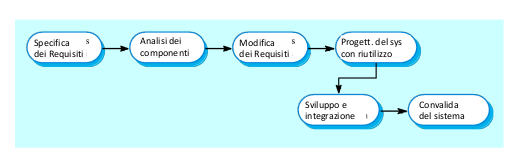
\includegraphics[scale=0.7]{img/ms.png}
\end{center}
Si ha ingegneria del software basata su componenti se si hanno già librerie su cui lavorare.\\
Passiamo al primo modello iterativo, quello di B. Boehm.
\begin{center}
	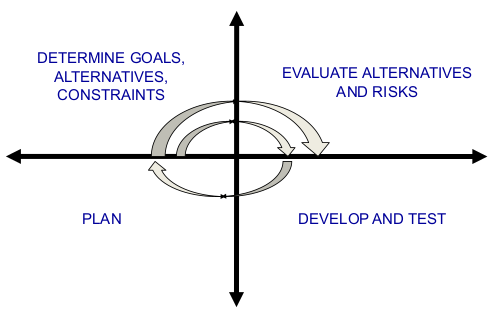
\includegraphics[scale=0.7]{img/ms2.png}
\end{center}
si parte dal quadrante in alto a sinistra e si arriva al prodotto finale mediante una serie di iterazioni. Si sceglie ovviamente la soluzione più sicura. I vari passaggi sono qui rappresentati:
\begin{center}
	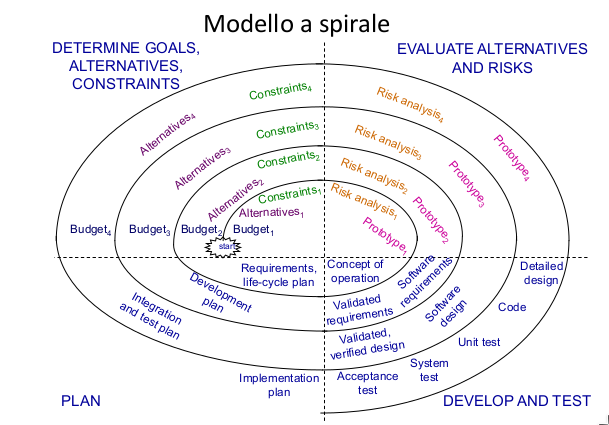
\includegraphics[scale=0.7]{img/ms3.png}
\end{center}
\section{Modello UP}
Il metodo di modellazione UP(Unified Process), conosciuto anche come RUP(Rational Unified Process), è un
processo iterativo molto diffuso per lo sviluppo software, in cui sono presenti degli elementi tratti da 
altri metodi, come Extreme Programming, Scrum e così via.

Lo sviluppo iterativo
Si hanno i modelli agili, che si basano sulla \textbf{consegna incrementale}. Si hanno iterazioni brevi e timeboxed, con un raffinamento evolutivo di piani, dei requisiti e del progetto. Questi metodi favoriscono la collaborazione nei gruppi e la riduzione dei costi.
\subsection{Modello UP o RUP}
Il metodo UP, \textit{inified process}, conosciuto anche come RUP, \textit{Rational Unified Process}, usa la notazione UML, \textit{unified modeling language} ed è uno dei più importanti modelli agili. È è un processo iterativo e incrementale. Si basa sulla suddivisone di un grande processo in iterazioni controllate. Si hanno passi piccoli, timeboxed da 2 a 6 settimane, feedback rapito e adattamento, di requisiti, modelli, stime di sviluppo e costi e priorità.
\begin{center}
	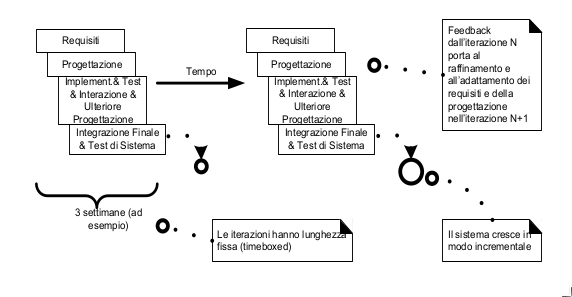
\includegraphics[scale=0.7]{img/ms4.png}
\end{center}
Si hanno 4 fasi nel modello RUP:
\begin{enumerate}
	\item \textbf{avviamento:} dove viene stabilita la “bussines rationale” del progetto e stabiliti gli obiettivi, stime dei costi e dei tempi. Si ha uno studio di fattibilità, \textit{Life-Cycle Objective Milestone}
	\item \textbf{elaborazione}: dove si raccolgono i requisiti in modo più dettagliato, si procede con l'analisi ad alto livello per stabilire l'architettura di base e vengono analizzati i rischi principali. Si hanno stime più affidabili: \textit{Life-Cycle Architecture Milestone}
	\item \textbf{costruzione} che consiste di molte iterazioni, e ad ogni iterazione viene costruita una parte del sistema che soddisfa un sottoinsieme di requisiti. Viene effettuato il testing e l'integrazione. Si ha la preparazione al rilascio: \textit{Initial Operational Capability Milestone}
	\item \textbf{transizione:} dove vengono affrontati tutti gli aspetti legati al fine-tuning delle funzionalità,
	      prestazioni, qualità, beta-testing, ottimizzazione, formazione degli
	      utenti,... È la \textit{Product Release Milestone}
\end{enumerate}
\begin{center}
	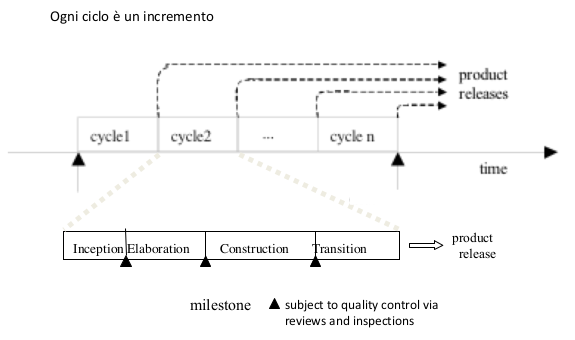
\includegraphics[scale=0.7]{img/ms5.png}
\end{center}
Si hanno i seguenti vantaggi dello sviluppo iterativo:
\begin{itemize}
	\item minore chance di fallimento del progetto
	\item riduzione precoce dei rischi
	\item progresso visibile
	\item feedback precoce e coinvolgimento dell'utente
	\item "abbracciare il cambiamento"
\end{itemize}
\begin{center}
	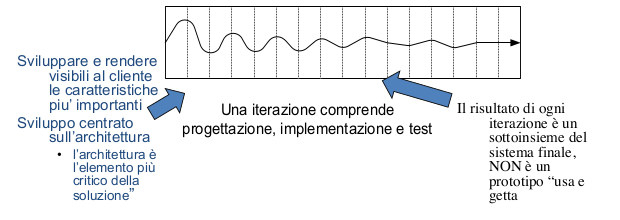
\includegraphics[scale=0.7]{img/ms6.png}
\end{center}
Vediamo un esempio con 5 iterazioni:
\begin{center}
	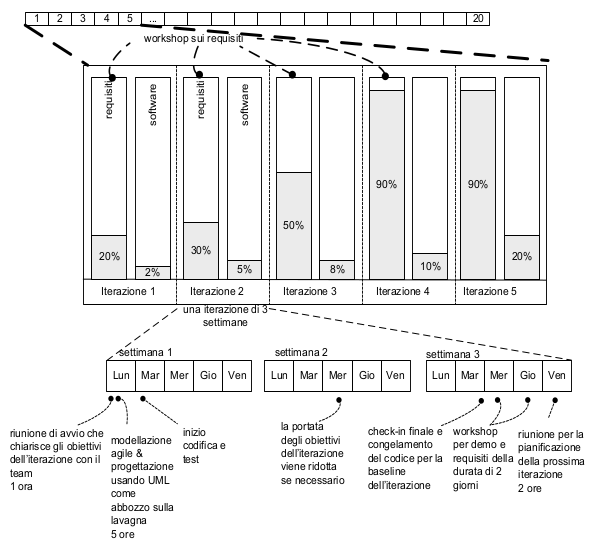
\includegraphics[scale=0.7]{img/ms7.png}
\end{center}
\newpage
vediamo un'altra rappresentazione del ciclo di sviluppo:
\begin{center}
	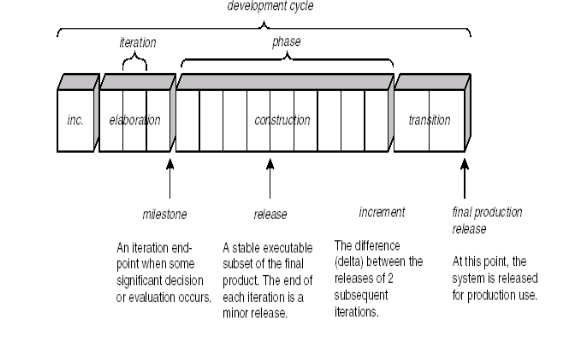
\includegraphics[scale=0.65]{img/ms8.png}
\end{center}
vediamo anche un'immagine per rappresentare l'organizzazione del processo, con fasi, iterazioni e "discipline":
\begin{center}
	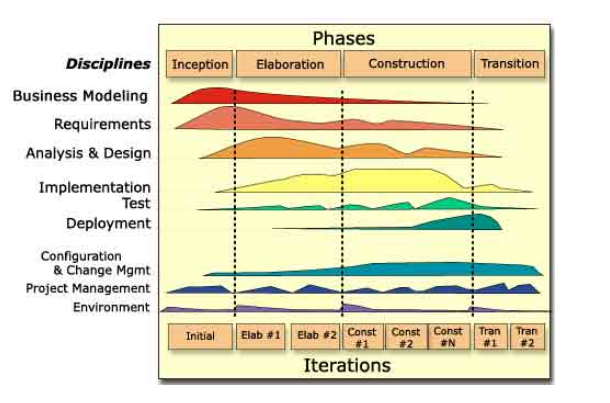
\includegraphics[scale=0.65]{img/ms9.png}
\end{center}
tra le discipline troviamo analisi e progettazione
%approfondire su libro
Si hanno le seguenti caratteristiche principlai per l?UP:
\begin{itemize}
	\item è iterativo e incrementale
	\item si enfasi sul modello invece che sul linguaggio naturale
	\item è centrato sull'architettura
\end{itemize}
\subsection{Processo Scrum}
Iniziamo con un'immagine che rappresenta questo metodo agile:
\begin{center}
	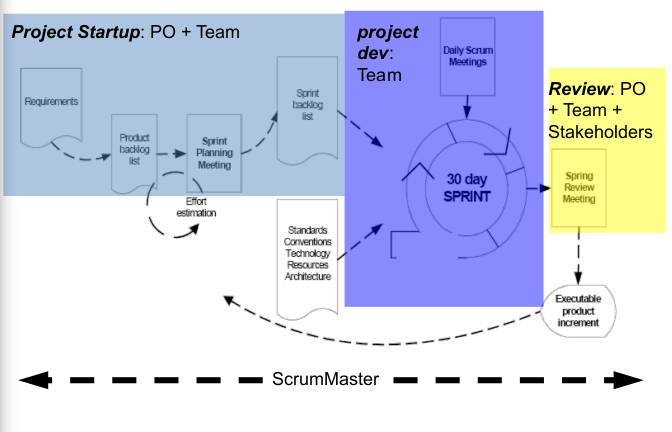
\includegraphics[scale=0.65]{img/ms10.png}
\end{center}
È un processo iterativo basato sull controllo dello stato di
avanzamento. Si hanno i seguenti principi fondamentali:
\begin{itemize}
	\item \textbf{visibilità:} gli aspetti significativi del processo di sviluppo devono essere visibili a tutti e tutti gli aspetti devono essere chiari
	\item \textbf{ispezione:} poter ispezionare frequentemente il lavoro fatto per verificare che si sta procedendo verso gli
	      obiettivi posti
	\item \textbf{adattamento}, se si sta deviando dagli obiettivi, occorre un adattamento per minimizzare altre deviazioni. Deve essere svolto nel minor tempo possibile in caso di necessità
\end{itemize}
Si hanno i seguenti ruoli:
\begin{itemize}
	\item \textbf{product owner} che si occupa della definizione delle
	      caratteristiche del progetto da sviluppare (1 sola
	      persona, e.g. committente, o altri...); gestisce il
	      Product Backlog. Lavora costantemente col team
	\item \textbf{team:} dedicato allo sviluppo e rilascio del
	      prodotto attraverso incrementi successivi (da 3 a
	      7/8 membri)
	\item \textbf{scrum master:} responsabile che lo SCRUM venga
	      applicato correttamente. Non è un project manager, fa da intermezzo tra team e product owner, collabora col team etc
\end{itemize}
Ecco un'immagine che rappresenta lo sviluppo con Scrum:
\begin{center}
	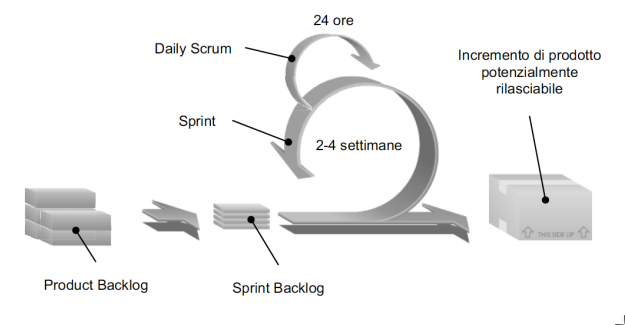
\includegraphics[scale=0.7]{img/ms11.png}
\end{center}
SI hanno quindi:
\begin{itemize}
	\item releases brevi con sottoinsiemi consegnati velocemente
	\item in ogni istante si hanno test eseguibili, non si ha logica duplicata e si ha un numero minimo di features
	\item si ha \textit{refactoring }con miglioramento continuo
	\item si un testo continuo e automatico, \textit{testing first}
	\item si hanno due sviluppatori che lavorano insieme, \textit{pair programming}
	\item il codice è proprietà del team e non del singolo dev, \textit{collective owbership}
	\item si hanno check-in frequenti e integrazioni continue, \textit{continuous integration}
	\item il cliente lavora col team
\end{itemize}
I \textbf{requisiti} sono una descrizione dei servizi del sistema e dei suoi vincoli operativi. Si hanno due tipi di requisiti:
\begin{itemize}
	\item \textbf{requisiti utenti:} affermazioni in linguaggio naturale, corredate da tabelle e diagrammi, riguardanti i servizi che il sistema offre ed i vincoli operazionali. Sono scritti per i clienti e sono da loro comprensibili anche se non	hanno conoscenze tecniche dettagliate.\\

	\item \textbf{requisiti di sistema:} un documento strutturato che definisce in modo dettagliato le funzioni del sistema, i servizi ed i vincoli operazionali. Definisce cosa deve essere implementato, quindi può essere parte del
	      contratto tra acquirente e sviluppatore. È la base del progetto della soluzione e può essere illustrato utilizzando i \textbf{modelli di sistema}.

\end{itemize}
i requisiti possono avere 3 problemi:
\begin{itemize}
	\item \textbf{ambiguità:} il sistema fornisce visualizzazioni appropriate per leggere i documenti
	\item \textbf{incompletezza:} i requisiti devono descrivere tutti i	servizi forniti dal sistema (anche se in realtà tutto ciò è impossibile, per questo esistono i cambiamenti)
	\item \textbf{inconsistenza}: le descrizioni non devono contenere conflitti o contraddizioni (anche questa cosa è difficilissima da ottenere)
\end{itemize}
SI hanno anche i \textbf{requisiti funzionali} servizi che il sistema deve (o non deve) fornire. Si hanno anche i \textit{requisiti non funzionali}, come vincoli sui servizi temporali, standard, sull'usabilità etc... I requisiti non funzionali possono essere più critici dei requisiti funzionali: \textbf{se non sono soddisfatti il sistema è spesso inutilizzabile}. Si hanno alcuni requisiti non funzionali:
\begin{itemize}
	\item \textbf{prodotto: }specificano che il prodotto deve comportarsi in un modo particolare
	      esempi: velocità di esecuzione, affidabilità.\\
	      \textit{L’interfaccia utente sarà implementata con HTML semplice senza frames
		      e applets}
	\item \textbf{organizzativi: }conseguenza di politiche e procedure dell’organizzazione del cliente e dello sviluppatore.
	      esempi: linguaggio di programmazione, metodo di sviluppo.\\
	      \textit{Il processo di sviluppo e la relativa documentazione sarà conforme alle
		      norme XYZCo-SP-STAN-95}
	\item \textbf{esterni: }provengono da fattori esterni al sistema e al processo di sviluppo.
	      esempi: interoperabilità, leggi e norme.
	      \\ \textit{Il sistema non deve rilevare agli operatori nessuna informazione
		      personale sui clienti oltre al nome e al numero di riferimento}
\end{itemize}
\begin{center}
	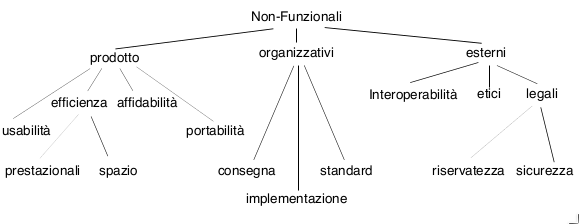
\includegraphics[scale=0.8]{img/req.png}
\end{center}
\newpage
Tutto ciò perché il linguaggio naturale presenta mancanza di chiarezza, ambiguità, confusione etc... Esistono alternative:
\begin{center}
	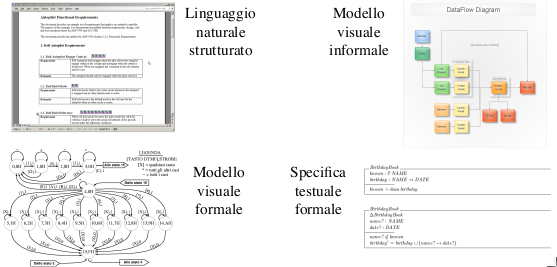
\includegraphics[scale=0.8]{img/req2.png}
\end{center}
I requisiti hanno un formato standard, usano il linguaggio in modo consistente, evitano il gergo tecnico e evidenziano delle porzioni di testo per identificare le parti più importanti dei requisiti. Un esempio di standard è quello IEEE830.\\
I casi d'uso possono essere visualizzati con l'UML:
\begin{center}
	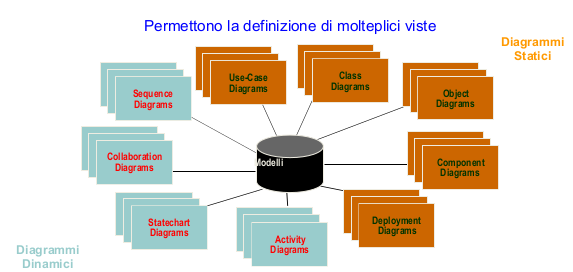
\includegraphics[scale=0.8]{img/uml.png}
\end{center}

\chapter{Casi d'uso}
\textit{I casi d'uso sono storie scritte, testuali, di qualche attore che usa un sistema per raggiungere degli obbiettivi}. I casi d'uso possono a loro volta influenzare molti altri elaborati dell'analisi, progettazione, implementazione, gestione del progetto e test. Passiamo a qualche definizione:
\begin{itemize}
	\item un \textbf{attore} è qualcosa 6 qualcuno dotato di
		comportamento, come una persona (caratterizzata da un ruolo), un sistema informatico o un'organizzazione
	\item uno \textbf{scenario o istanza di caso d'uso} è una sequenza specifica di azioni e interazioni
		  tra il sistema e alcuni attori. Uno scenario descrive una particolare storia nell'uso del sistema, o un percorso attraverso il caso d'uso
\end{itemize}
\textit{Informalmente }un caso d'uso quindi può essere definito come una collezione di scenari correlati, di successo e fallimento, che descrivono un attore che usa un sistema per raggiungere un obiettivo.\\
\textbf{UP} definisce il modello di caso nell'ambito della disciplina dei Requisiti. Inoltre \textbf{i casi d'uso sono documenti di testo, non diagrammi, e la modellazione dei casi
d'uso è innanzitutto un atto di scrittura di testi, non di disegno di diagrammi}. Il Modello dei Casi d'Uso può includere, opzionalmente, un diagramma UML dei casi
d'uso che mostra i nomi dei casi d'uso e degli attori, nonché le relazioni tra di essi. Esso costituisce un buon diagramma di contesto di un sistema e del suo ambiente, oltre a
costituire un indice di facile consultazione dei nomi dei casi d'uso. Si ricorda che \textbf{i casi d'uso non sono orientati ad oggetti}.\\
I casi d'uso sono un buon metodo per mantenere la semplicità e consentire agli esperti
di dominio o ai fornitori di requisiti di scrivere essi stessi i casi d'uso, o perlomeno partecipare alla loro scrittura. Un altro valore dei casi d'uso è che mettono in risalto gli obiettivi e il punto di vista
dell'utente.\\
I casi d'uso sono requisiti, soprattutto requisiti funzionali o comportamentali, che indicano che cosa farà il sistema. In UP e in molti metodi moderni, i casi d'uso sono il meccanismo
centrale che viene consigliato per la scoperta e la definizione dei requisiti.\\
Torniamo a parlare di attori. Un attore è qualcosa o qualcuno dotato di comportamento, Anche il sistema in discussione,\textit{ SuD, da system under discussion}, stesso è un attore, quando ricorre ai servizi di altri sistemi. Si hanno tre tipi di attori correlati al SuD:
\begin{enumerate}
	\item \textbf{attore primario} che raggiunge degli obiettivi utente utilizzando i servizi del SuD. Identificare gli attori primari è utile per trovare gli obiettivi degli utenti,che guidano i casi d'uso
	\item \textbf{attore di supporto} che offre un servizio (per esempio, informazioni) al SuD. Spesso è un sistema informatico, ma potrebbe essere un'organizzazione o una
	persona. Identificare gli attori di supporto è utile per chiarire le interfacce esterne e i loro protocolli
	\item \textbf{attore fuori scena} che ha un interesse nel comportamento del caso d'uso, ma non è
	un attore primario o di supporto. Identificare gli attori fuori scena è utile per garantire che tutti gli interessi necessari vengano individuati e soddisfatti. Gli interessi degli attori fuori scena sono spesso sottili o facili da tralasciare, a meno che gli attori stessi non vengano esplicitamente nominati
\end{enumerate}
Si hanno inoltre tre diversi livelli di \textbf{formalità} per i casi d'uso:
\begin{enumerate}
	\item \textbf{formato breve} ovvero un riepilogo conciso di un solo paragrafo, normalmente relativo al
	solo scenario principale di successo. Si usa durante l'analisi iniziale dei requisiti, per capire rapidamente l'argomento e la portata. È possibile scriverlo in pochi minuti
	\item \textbf{formato informale} ovvero più paragrafi, scritti in modo informale, relativi a vari scenari. Si usa come il formato breve ma qui si ha un livello di dettaglio maggiore
	\item \textbf{formato dettagliato} dove tutti i passi e le variazioni sono scritti nel dettaglio; ci sono anche delle sezioni di supporto, come le pre-condizioni e le garanzie di successo. Va usato opo che molti casi d'uso sono stati identificati e scritti in formato breve, alcuni casi d'uso (circa il 10\%) che hanno maggior valore e che sono più significativi dal punto di vista dell'architettura vengono scritti in formato dettagliato. Si ha quindi:
	\begin{center}
		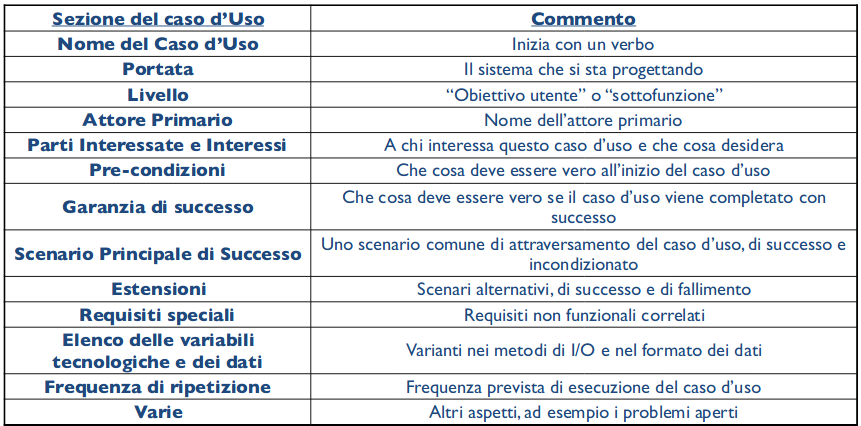
\includegraphics[scale=0.5]{img/det.png}
	\end{center}
\end{enumerate}
Parliamo ora di scenari. Si hanno due tipologie:
\begin{enumerate}
	\item \textbf{scenario principale (di successo)} che descrive un percorso di successo tipico che soddisfa gli interessi delle parti interessate. Si noti che spesso non comprende alcuna condizione o diramazione. Questo rende il caso d'uso più comprensibile e più estensibile. È formato da una sequenza di passi:
	\begin{enumerate}
		\item un'interazione tra attori
		\item una validazione (solitamente effettuata dal sistema
		\item un cambiamento di stato da parte del sistema
	\end{enumerate}
	Il primo passo di un caso d'uso non rientra sempre in questa classificazione, ma può indicare l'evento (trigger) che scatena l'esecuzione dello scenario. I nomi degli attori vengono di solito scritti con l'iniziale maiuscola, per facilitarne l'identificazione. Un esempio:
	\begin{center}
		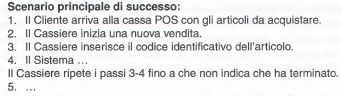
\includegraphics[scale=1.1]{img/pri.png}
	\end{center}
	\item \textbf{scenari alternativi (o flussi alternativi o estensioni)} che descrivono tutte le diramazioni e gli altri scenari, sia di successo che di fallimento. La loro stesura è spesso lunga e complessa. Nella scrittura completa dei casi d'uso, la combinazione del flusso di base e degli altri scenari descritti dalle estensioni dovrebbe soddisfare "quasi" tutti gli interessi delle parti interessate. Tuttavia, alcuni interessi possono essere descritti come requisiti non funzionali, e pertanto riportati nelle Specifiche Supplementari piuttosto che nei casi d'uso. Gli scenari relativi alle estensioni sono diramazioni dello scenario principale di successo, e vengono indicati con riferimento ai suoi passi. Si contrassegnano con una lettera posta dopo il numero che identifica il passo (per il passo 3 si avrà 3a, 3b etc...) inoltra prima riporta la condizione, poi la reazione. Per esempio:
	\begin{center}
		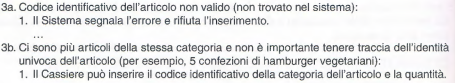
\includegraphics[scale=0.9]{img/alt.png}
	\end{center}
	Un estensione è costituita da condizione e gestione. La gestione di un'estensione può essere riassunta in un unico passo, oppure può comprendere una sequenza di passi. Al termine della gestione di un'estensione, per default lo scenario si fonde di nuovo con lo scenario principale di successo, a meno che l'estensione non indichi diversamente (per esempio, l'arresto del sistema). In alcuni casi, i punti di estensione sono abbastanza complessi. Questo può essere un motivo per esprimere l'estensione come un caso d'uso separato.
\end{enumerate}
Un caso d'uso può diramarsi in un altro caso d'uso e in effetti, i casi d'uso vengono spesso scritti come ipertesti, e l'esecuzione di un altro caso d'uso viene rappresentata come un collegamento ipertestuale. In questo caso, facendo clic sul nome del caso d 'uso sottolineato, ne verrà visualizzato il testo.\\
Se un requisito non funzionale, un attributo di qualità o un vincolo si riferiscono in modo specifico a un caso d' uso, allora è bene registrarlo insieme al caso d'uso. Potrebbe trattarsi di qualità come prestazioni, affidabilità e usabilità, oppure di vincoli di progettazione, che siano stati imposti o considerati probabili. Si hanno quindi i \textbf{requisiti speciali}.
\newpage
Vediamo ora un esempio completo di caso d'uso:
\begin{center}
	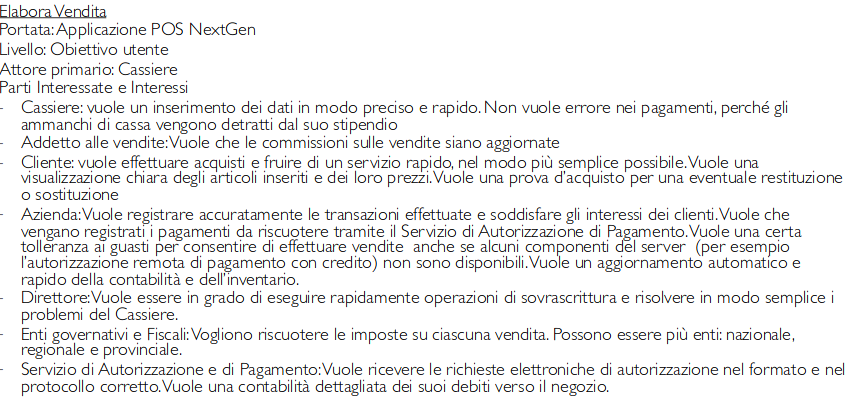
\includegraphics[scale=0.57]{img/ca1.png}
\end{center}
\begin{center}
	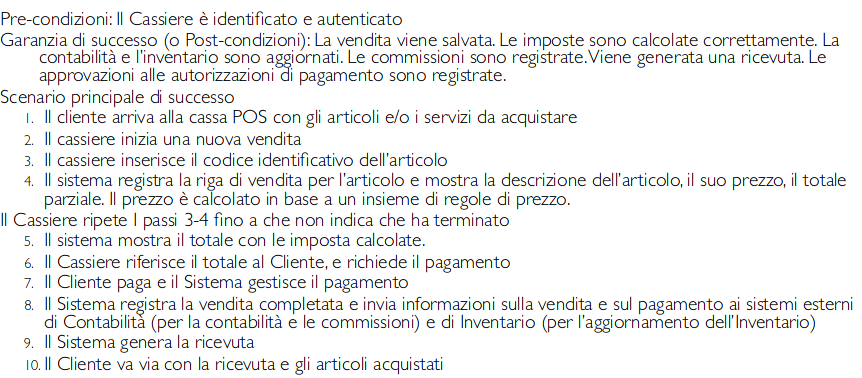
\includegraphics[scale=0.57]{img/ca2.png}
\end{center}
\begin{center}
	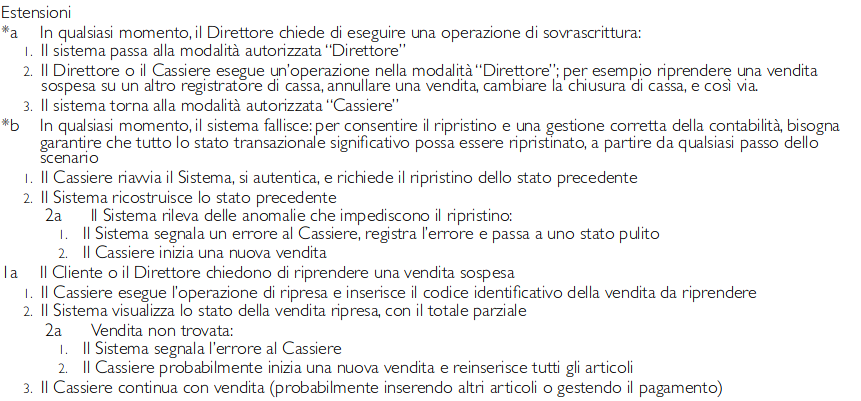
\includegraphics[scale=0.57]{img/ca3.png}
\end{center}
\begin{center}
	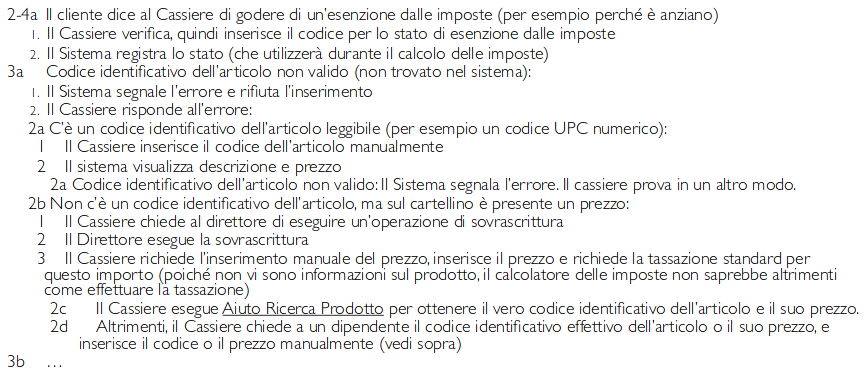
\includegraphics[scale=0.57]{img/ca4.png}
\end{center}
\begin{center}
	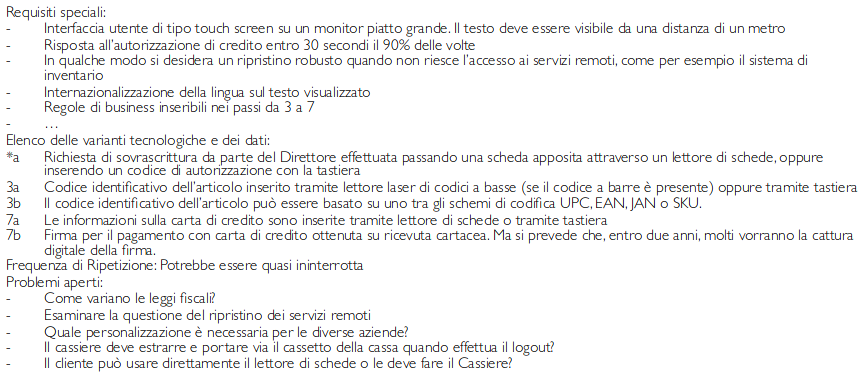
\includegraphics[scale=0.57]{img/ca5.png}
\end{center}
Si hanno delle linee guida per la stesura dei casi d'uso. Si cerca uno stile essenziale, ignorando l'interfaccia utente e concentrandosi sullo scopo dell'attore, ignorando come un sistema fa qualcosa ma concentrandosi su cosa deve fare. Per facilitare la lettura dei requisiti, è perciò opportuno scrivere i casi d'uso in modo conciso, e allo stesso tempo in modo completo (con una chiara indicazione di soggetto  verbo e di eventuali frasi subordinate).\\
I \textbf{casi d'uso a scatola nera }sono il tipo più comune e consigliato; non descrivono il funzionamento interno del sistema, i suoi componenti o aspetti relativi al suo progetto. Piuttosto, il sistema è descritto come dotato di responsabilità. Questa è una metafora comune e unificante nel pensare orientato agli oggetti; gli elementi software hanno responsabilità e collaborano con altri elementi dotati di responsabilità. Usando i casi d'uso a scatola nera per definire le responsabilità del sistema, è possibile specificare che cosa deve fare il sistema (comportamento o requisiti funzionali) senza decidere come lo farà (progettazione). In effetti, la definizione dell'"analisi" rispetto alla "progettazione" è talvolta riassunta come "che cosa" rispetto a "come". Questo è un tema importante nello sviluppo del software: durante l'analisi dei requisiti bisogna specificare il comportamento esterno del sistema, considerato a scatola nera, evitando di prendere decisioni sul "come". Successivamente, durante la progettazione, andrà creata una soluzione che soddisfa le specifiche. 
\newpage
Per esempio:
\begin{center}
	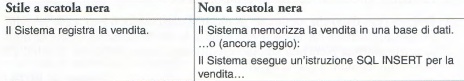
\includegraphics[scale=0.7]{img/box.png}
\end{center}
È anche importante trovare i casi d'uso e si ha una procedura di base per farlo:
\begin{enumerate}
	\item scegliere i confini del sistema, ovvero definire il sistema al meglio. Per chiarire la definizione dei confini del sistema in corso di progettazione, è utile sapere che gli attori primari e gli attori di supporto sono considerati esterni al sistema. Una volta identificati gli attori esterni, i confini diventano più chiari.
	\item identificare gli attori primari. Alcune volte sono gli obiettivi a svelare gli attori, o viceversa. Si possono usare una serie di domande per facilitare l'operazione:
	\begin{center}
		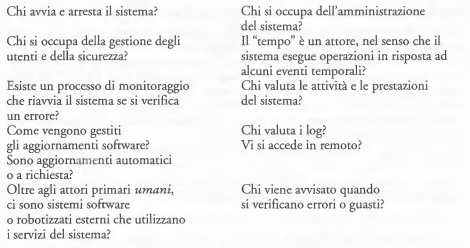
\includegraphics[scale=0.7]{img/dom.png}
	\end{center}
	\item identificare gli obiettivi di ciascun attore primario. Si crea quinid un elenco attori-obiettivi, tipo questo:
	\begin{center}
		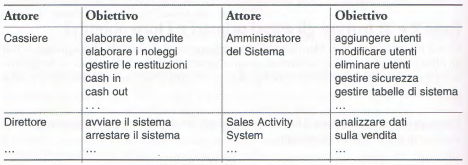
\includegraphics[scale=0.7]{img/atob.png}
	\end{center}
	inoltre risulta più producente, nella realtà, chiedere all'attore stesso quale sia il suo obbiettivo. \\
	Un altro approccio per trovare attori, obiettivi e casi d'uso è basato sull'identificazione di eventi esterni. Spesso un gruppo di eventi appartiene allo stesso caso d'uso. Per esempio:
	\begin{center}
	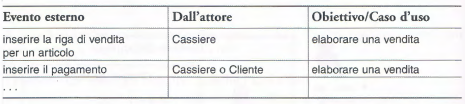
\includegraphics[scale=0.7]{img/atob2.png}
	\end{center}
	\item definire i casi d'uso che soddisfano gli obiettivi degli utenti; il loro nome va scelto in base all'obiettivo. Di solito, i casi d'uso a livello di obiettivo utente saranno in corrispondenza biunivoca con gli obiettivi degli utenti. 
\textbf{Il nome dei casi d'uso deve iniziare con un verbo e, in generale va definito un caso d'uso per ciascun obiettivo utente.} È opportuno assegnare al caso d'uso un nome simile all'obiettivo dell'utente. \\ \textit{un'eccezione comune alla scelta di un caso d'uso per obiettivo è quella che riunisce gli obiettivi separati CRUD (acronimo di create, retrieve, update, delete, ovvero creare, leggere, aggiornare, eliminare) in un unico caso d'uso CRUD, chiamato Gestisci <X>. Per esempio, gli obiettivi "modifica utente" , "elimina utente" e così via sono tutti soddisfatti dal caso d'uso Gestisci Utenti.}
\end{enumerate}
\textbf{Naturalmente, nello sviluppo iterativo ed evolutivo, non tutti gli obiettivi o i casi d'uso
saranno identificati completamente o correttamente fin dall'inizio. Anche la scoperta dei
requisiti è evolutiva}.\\
Bisogna poi verificare la validità dei casi d'uso. Si hanno quindi tre test:
\begin{itemize}
	\item \textbf{test del capo}: \textit{il capo vi chiede: "Cosa avete fatto tutto il giorno?" e voi rispondete: "Il login!". Il vostro capo sarà felice?}. Se non lo è il caso d'uso non supera il test del capo, il che significa che non è fortemente mirato a ottenere risultati il cui valore sia misurabile. Potrebbe essere un caso d'uso a un livello più basso, ma non al livello a cui è desiderabile concentrarsi durante l'analisi dei requisiti. Ciò non significa che bisogna sempre ignorare i casi d'uso che non superano il test del capo
	\item \textbf{test EBP (\textit{Elementary Business Process})}, che deriva dall'ingegneria dei processi di business: \textit{Un processo di business elementare è un'attività svolta da una persona in un determinato tempo e luogo, in risposta a un evento di business, che aggiunge un valore di business misurabile e lascia i dati in uno stato coerente; per esempio, "Approva un credito" o "Stabilisci il prezzo per un ordine"}. Come nella definizione di UP, enfatizza l'aggiunta di un valore di business osservabile o misurabile, e giunge a una situazione in cui il sistema e i dati sono in uno stato stabile e coerente. \textbf{Il test EBP è simile al test del capo, soprattutto in termini di qualifica in termini di valore aziendale misurabile.}
	\item \textbf{test della dimensione}, che si basa sul fatto che un caso d'uso è formato da diversi passi (e nel complesso si hanno da 3 a 10 pagine di testo). Un errore comune nella modellazione dei casi d'uso è definire un caso d'uso a sé formato da un singolo passo.
\end{itemize}
\textbf{Ci potrebbero essere delle eccezioni a questi test.}
\section{Diagrammi dei casi d'uso}
UML fornisce una notazione dei diagrammi dei casi d'uso che consente di illustrare i nomi e gli attori dei casi d'uso, nonché le relazioni tra gli stessi, per esempio:
\begin{center}
	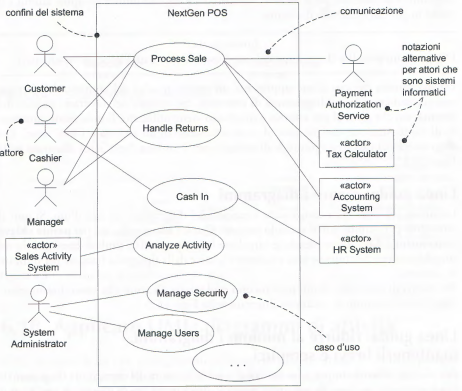
\includegraphics[scale=0.7]{img/casd.png}
\end{center}
\newpage
\textbf{I diagrammi dei casi d'uso e le relazioni tra casi d'uso sono secondari nel lavoro che
riguarda i casi d'uso. I casi d'uso sono documenti di testo. Lavorare sui casi d'uso significa scrivere testo.} \\
Un diagramma dei casi d'uso rappresenta un ottimo quadro del contesto del sistema; esso costituisce un buon diagramma di contesto, che consiste nel mostrare i confini del sistema, ciò che giace al suo esterno e come esso viene utilizzato. È utile come strumento di comunicazione che riassume il comportamento di un sistema e i suoi attori.\\
\textit{Per ribadire, il lavoro importante dei casi d'uso è la scrittura del testo, non i diagrammi o le relazioni tra casi d'uso. Se un'organizzazione spreca molte ore (o peggio ancora, giorni) a lavorare su un diagramma dei casi d' uso e a discutere le relazioni tra casi d'uso anziché concentrarsi sulla scrittura del testo, vuol dire che il tempo è stato impiegato male}.\\
A livello di notazione si ha:
\begin{itemize}
	\item \textbf{gli attori} sono rappresentati da un omino, col nome scritto sotto:
	\begin{center}
		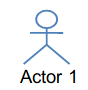
\includegraphics[scale=0.7]{img/act.png}
	\end{center}
	\item \textbf{i casi d'uso} sono rappresentati con un ovale contenente la dicitura del caso d'uso:
	\begin{center}
		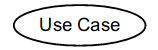
\includegraphics[scale=0.7]{img/dcas.png}
	\end{center}
	\newpage
	\item \textbf{le associazioni} sono canali di comunicazione tra attore e caso d'uso. Si hanno due rappresentazioni:
	\begin{enumerate}
		\item \textbf{una linea continua direzionata}, per specificare chi da inizio all'interazione
		\item \textbf{una linea continua non direzionata}, per indicare che entrambe le parti possono dare inizio ad un'interazione
	\end{enumerate}
	\begin{center}
		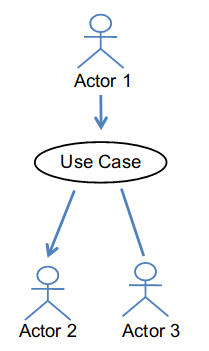
\includegraphics[scale=0.7]{img/asso.png}
	\end{center}
	\item \textbf{l'include (inclusione)} si rappresenta con una linea tratteggiata direzionata con l'indicazione \textit{<<include>>} e indica la relazione tra un caso d'uso base ed un caso d'uso incluso nel caso d'uso base:
	\begin{center}
		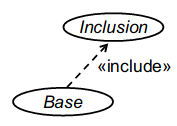
\includegraphics[scale=0.7]{img/incd.png}
	\end{center}
	\begin{center}
		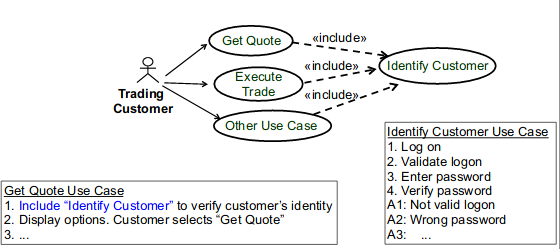
\includegraphics[scale=0.7]{img/incd2.png}
	\end{center}
	\textit{il caso d'uso è eseguito completamente quando viene raggiunto il punto di inclusione}
	\item \textbf{l'extend (estensione)}, si rappresenta come l'include (specificando \textit{<<extend>>}) e connette un caso d'uso esteso ad un caso d'uso base. Aggiunge varianti ad un caso d’uso base e viene inserito solo se la condizione di estensione è vera. Si hanno estensioni inserite solo in corrispondenza degli extension point:
	\begin{center}
		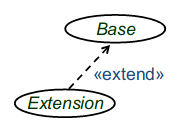
\includegraphics[scale=0.7]{img/extd.png}
	\end{center}
	\begin{center}
		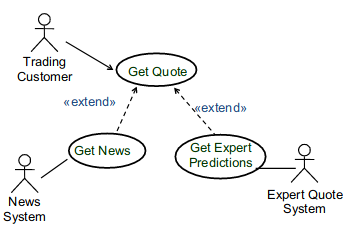
\includegraphics[scale=0.7]{img/extd2.png}
	\end{center}
	\begin{center}
		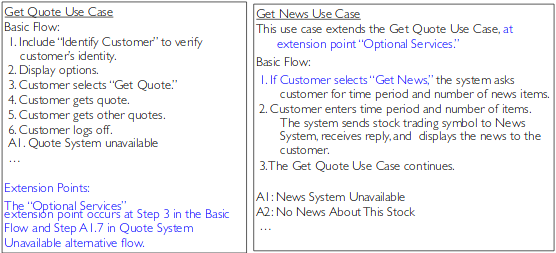
\includegraphics[scale=0.7]{img/extd3.png}
	\end{center}
	\textit{Il caso d'uso esteso è eseguito quando il punto di estensione è raggiunto e la condizione di estensione è vera}
	\item \textbf{la generalization (generalizzazione)} si ha quando un caso d'uso base è una generalizzazione di un caso d'uso child. Viene rappresentata con una linea continua direzionata con la freccia non riempita:
	\begin{center}
		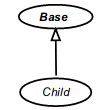
\includegraphics[scale=0.7]{img/gend.png}
	\end{center}
	\textit{Il caso d'uso generalizzato viene eseguito se la condizione di generalizzazione è vera} inoltre \textit{la generalizzazione è puramente concettuale, non ci sono regole da seguire, come ad esempio l'utilizzo di punti di estensione}. Si ha:
	\begin{center}
		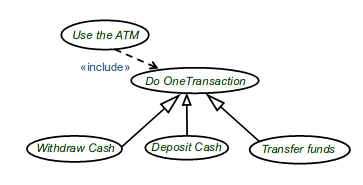
\includegraphics[scale=0.7]{img/gend2.png}
	\end{center}\begin{center}
		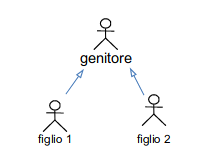
\includegraphics[scale=0.7]{img/gend3.png}
	\end{center}\begin{center}
		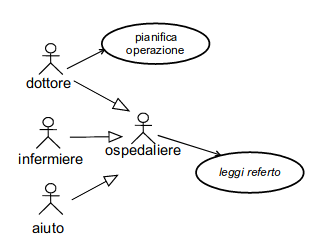
\includegraphics[scale=0.7]{img/gend4.png}
	\end{center}
	
\end{itemize}
\begin{shaded}
Anche se gli elenchi dettagliati di funzioni non sono consigliabili, le funzionalità del
sistema possono essere riassunte in modo utile in un \textit{elenco di caratteristiche} chiaro, ad
alto livello, chiamato caratteristiche di sistema, come parte del documento di Visione. Contrariamente alle caratteristiche di basso livello, costituite da molte pagine, un elenco di caratteristiche di sistema dovrebbe comprende solo alcune decine di voci. Esso fornisce un riepilogo conciso delle funzionalità del sistema, indipendente dalla vista dei casi d'uso, come nel seguente esempio. Talvolta i casi d'uso non sono adatti; alcune applicazioni richiedono un punto di vista guidato dalle caratteristiche. Per esempio, i server applicativi, i sistemi di gestione di basi di dati e altri sistemi di middleware o di back-end vanno piuttosto descritti e si evolvono in termini di caratteristiche ("supporto per i Web Services nella prossima versione"). I casi d'uso non sono idonei a queste applicazioni o al modo in cui esse~evolvono in termini di forze del mercato.
\end{shaded}
\newpage
I casi d'uso sono fondamentali in UP e in molti altri metodi iterativi. UP incoraggia lo sviluppo guidato dai casi d'uso. Si ha quindi:
\begin{itemize}
	\item i requisiti funzionali sono registrati principalmente nei casi d'uso (Modello dei Casi d'Uso); le altre tecniche per i requisiti (come l'elenco delle funzioni) sono secondarie, o addirittura non utilizzate
	\item i casi d'uso rivestono un ruolo importante nella pianificazione iterativa. Il lavoro di un'iterazione è definito, in parte, scegliendo alcuni scenari di casi d'uso o interi casi d'uso. I casi d'uso sono inoltre un input fondamentale per stimare costi e tempi di un progetto
	\item la progettazione è guidata da realizzazioni di casi d'uso; il team progetta oggetti e sottosistemi che collaborano che consentono di eseguire o realizzare i casi d'uso
	\item i casi d'uso spesso influenzano l'organizzazione dei manuali per l'utente
	\item i test funzionali o di sistema corrispondono agli scenari dei casi d'uso
	\item è possibile creare nella UI "creazioni guidate" (wizard) o scelte rapide (shortcut) per facilitare le attività comuni degli scenari dei casi d'uso più comuni e importanti
\end{itemize}
\chapter{Contratti delle Operazioni}
In UP, i \textbf{casi d'uso} e le \textbf{caratteristiche di sistema} sono i modi principali per descrivere il comportamento del sistema. Normalmente sono sufficienti, ma talvolta è utile una descrizione più dettagliata o precisa del comportamento del sistema. I contratti delle operazioni usano pre-condizione e post-condizione per descrivere nel dettaglio i cambiamenti agli oggetti in un modello di dominio, come risultato di un'operazione di sistema.\\
I contratti delle operazioni possono essere considerati parte del Modello dei Casi d'Uso, poiché forniscono maggiori dettagli dell'analisi sull'effetto delle operazioni di sistema implicate dai casi d'uso.\\
Definiamo le sezioni di un contratto:
\begin{itemize}
	\item \textbf{operazione:} nome e parametri dell'operazione
	\item \textbf{riferimenti:} casi d'uso in cui può verificarsi questa operazione
	\item \textbf{pre-condizioni: }ipotesi significative sullo stato del sistema o degli oggetti nel Modello di Dominio prima dell'esecuzione dell'operazione. Sono ipotesi non banali.
	\item \textbf{post-condizioni: }è la sezione più importante ovvero lo stato degli oggetti nel Modello di Dominio dopo il completamento dell'operazione. Le post-condizioni descrivono i cambiamenti nello stato degli oggetti nel modello di dominio. I cambiamenti di stato nel modello di dominio comprendono le istanze create, le associazioni formate o rotte e gli attributi modificati. Le post-condizioni non sono azioni da eseguire nel corso dell'operazione; si tratta piuttosto di osservazioni (rilevazioni) sugli oggetti del modello di dominio che risultano avere al termine dell'operazione. Si dividono in:
	\begin{itemize}
		\item creazione o cancellazione di un'istanza
		\item cambiamento del valore di un attributo
		\item associazioni (collegamenti in UML) formate o spezzate
	\end{itemize}
	\textbf{Le post-condizioni non sono sempre necessarie}. \textit{Le post-condizioni vanno espresse con un verbo al passato, per sottolineare che si tratta di osservazioni dei cambiamenti di stato provocati da un'operazione, e non di un'azione che deve accadere}
\end{itemize}
I contratti delle operazioni possono essere definiti per le \textbf{operazioni di sistema}, ovvero operazioni che il sistema, considerato come un componente a scatola nera, offre nella sua interfaccia pubblica. Le operazioni di sistema possono essere identificate mentre si abbozzano gli SSD, \textit{diagrammi di sequenza di sistema}.
\newpage
Un evento di sistema di input implica che il sistema contenga un'operazione di sistema per gestire quell'evento,
così come un messaggio OO (che è un tipo di evento o segnale) viene gestito da un metodo OO (che è un tipo di operazione):
\begin{center}
	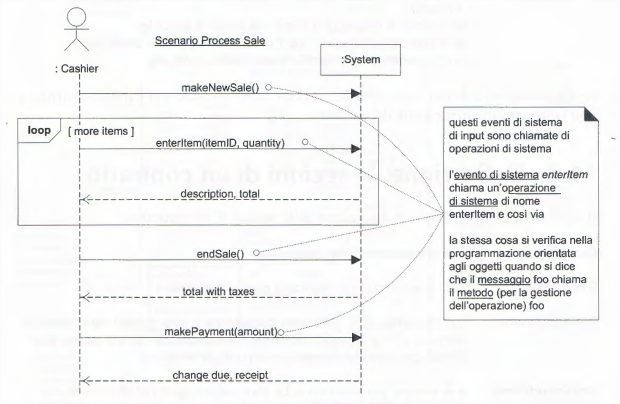
\includegraphics[scale=0.7]{img/oo.png}
\end{center}
L'intero insieme delle operazioni di sistema, tra tutti i casi d'uso, definisce l'interfaccia
di sistema pubblica, considerando il sistema come un singolo componente o una singola classe. In UML, il sistema nel suo insieme può essere rappresentato come un unico oggetto di una classe denominata, per esempio, System.\\
Durante la creazione dei contratti è normale che emerga la necessità di registrare nuove classi concettuali, attributi o associazioni nel modello di dominio. Non ci si limiti alla formulazione fatta in precedenza del modello di dominio; la si deve ampliare man mano che si fanno nuove scoperte.Nei metodi iterativi ed evolutivi (che riflettono la realtà dei progetti software), tutti gli elaborati dell'analisi e della progettazione sono considerati parziali e imperfetti, ed evolvono in risposta a nuove scoperte.\\
In UP, i casi d'uso sono il repository principale dei requisiti del progetto. Essi possono fornire tutti i dettagli, o la maggior parte di essi, necessari per sapere che cosa fare durante la progettazione; in questo caso i contratti non sono d'aiuto. Tuttavia ci sono situazioni in cui non è opportuno descrivere nei casi d' uso tutti i dettagli e la complessità dei cambiamenti di stato richiesti, poiché risulterebbero troppo dettagliati.
\\
Si ha la seguente linea guida per creare contratti:
\begin{itemize}
	\item identificare le operazioni di sistema dagli SSD
	\item creare un contratto per le operazioni di sistema complesse o i cui effetti sono probabilmente sottili, o che non sono chiare dai casi d'uso
	\item descrivere le post-condizioni con le seguenti categorie:
	\begin{itemize}
		\item creazione o cancellazione di istanza
		\item modifica di attributo
		\item associazione formata o spezzata
	\end{itemize}
\end{itemize}
\textit{Il problema più comune è dimenticarsi di includere la formazione di associazioni. In particolare quando sono creare nuove istanze, è molto probabile che debbano essere stabilire delle associazioni con diversi oggetti.}\\
\section{Operazioni e UML}
UML definisce formalmente la nozione di \textbf{operazione}: \textit{un'operazione è una specifica di una trasformazione o di una interrogazione che un oggetto può essere chiamato ad eseguire.}\\
In UML sono operazioni, per esempio, gli elementi di un'interfaccia. Sono quindi \textbf{astrazioni} e non implementazioni. In UML, invece, un \textbf{metodo} è:
\textit{l'implementazione di un'operazione. Esso specifica l'algoritmo o la procedura associata a un'operazione}.\\
Nel metamodello di UML, un'operazione ha una \textbf{firma} (o signature, con nome e parametri) e, cosa più importante in questo contesto, è associata a un insieme di oggetti UML di tipo Constraint (Vincolo) classificati come pre-condizioni e post-condizioni che specificano la semantica dell'operazione.
UML definisce la semantica delle operazioni attraverso i vincoli, che possono essere specificati nello stile delle pre-condizioni e post-condizioni. Si noti che, come sottolineato in questo capitolo, la specifica di un'operazione UML non può mostrare un algoritmo o una soluzione, ma solo i cambiamenti di stato o gli effetti dell'operazione. Oltre a utilizzare i contratti per specificare le operazioni pubbliche dell'intero sistema (ovvero, le operazioni di sistema), i contratti possono essere applicati alle operazioni a qualsiasi livello di granularità: le operazioni pubbliche (o l'interfaccia) di un sottosistema, di un componente, di una classe astratta, e così via. Per esempio, è possibile definire operazioni per una singola classe software, per esempio Stack. Le operazioni a grana grossa discusse in questo capitolo appartengono a una classe System che rappresenta l'intero sistema considerato come componente a scatola nera, ma in UML le operazioni possono appartenere a qualsiasi classe o interfaccia, tutte con le relative pre-condizioni e post-condizioni.
\end{document}
